% !TEX root = ../presentation.tex

\begin{frame}{Component Taxonomy: Passive vs. Active Devices}
    \begin{columns}[T]
        \begin{column}{0.48\textwidth}
            \begin{block}{Passive Components}
                \textit{Cannot introduce net electrical energy or amplify.}
                \begin{itemize}
                    \item \textbf{Resistors ($R$):} Dissipate energy as heat ($P = I^2 R$).
                    \item \textbf{Capacitors ($C$):} Store energy in electric field ($E = \frac{1}{2}CV^2$).
                    \item \textbf{Inductors ($L$):} Store energy in magnetic field ($E = \frac{1}{2}LI^2$).
                \end{itemize}
            \end{block}
        \end{column}
        \begin{column}{0.48\textwidth}
            \begin{exampleblock}{Active Components}
                \textit{Require external DC bias; can amplify or switch.}
                \begin{itemize}
                    \item \textbf{Diodes / LEDs:} Unidirectional conduction ($V > V_F$).
                    \item \textbf{BJTs:} Current-controlled current source ($I_C = \beta I_B$).
                    \item \textbf{MOSFETs:} Voltage-controlled channel switching.
                    \item \textbf{ICs:} Monolithic integration of micro-circuits.
                \end{itemize}
            \end{exampleblock}
        \end{column}
    \end{columns}
\end{frame}

\begin{frame}{Resistors: Color Codes \& Power Ratings}
    \begin{columns}[c]
        \begin{column}{0.48\textwidth}
            \begin{block}{Function \& Sizing}
                \begin{itemize}
                    \item Current limitation and potential division ($V = IR$).
                    \item Physical size correlates with \textbf{thermal power dissipation}, not resistance value!
                    \item Standard lab: $1/4\,\text{W}$ carbon/metal film.
                    \item High power: $1\,\text{W}, 2\,\text{W}$, up to $5\,\text{W}$ ceramic block.
                \end{itemize}
            \end{block}
        \end{column}
        \begin{column}{0.48\textwidth}
            \centering
            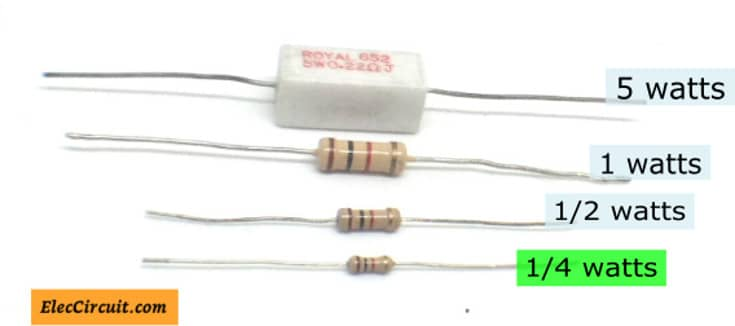
\includegraphics[width=\textwidth]{figures/fig_resistors.jpg}
        \end{column}
    \end{columns}
\end{frame}

\begin{frame}{Capacitors \& Inductors: Energy Storage}
    \begin{columns}[c]
        \begin{column}{0.48\textwidth}
            \begin{block}{Capacitor Types \& Polarity Danger}
                \begin{itemize}
                    \item \textbf{Ceramic (Non-polarized):} High frequency bypass ($10\,\text{pF}\text{--}100\,\text{nF}$).
                    \item \textbf{Electrolytic (Polarized):} High capacitance bulk filtering ($1\,\mu\text{F}\text{--}4700\,\mu\text{F}$).
                    \item \alert{Reverse polarity on electrolytics causes catastrophic electrolyte boiling and venting!}
                \end{itemize}
            \end{block}
        \end{column}
        \begin{column}{0.48\textwidth}
            \centering
            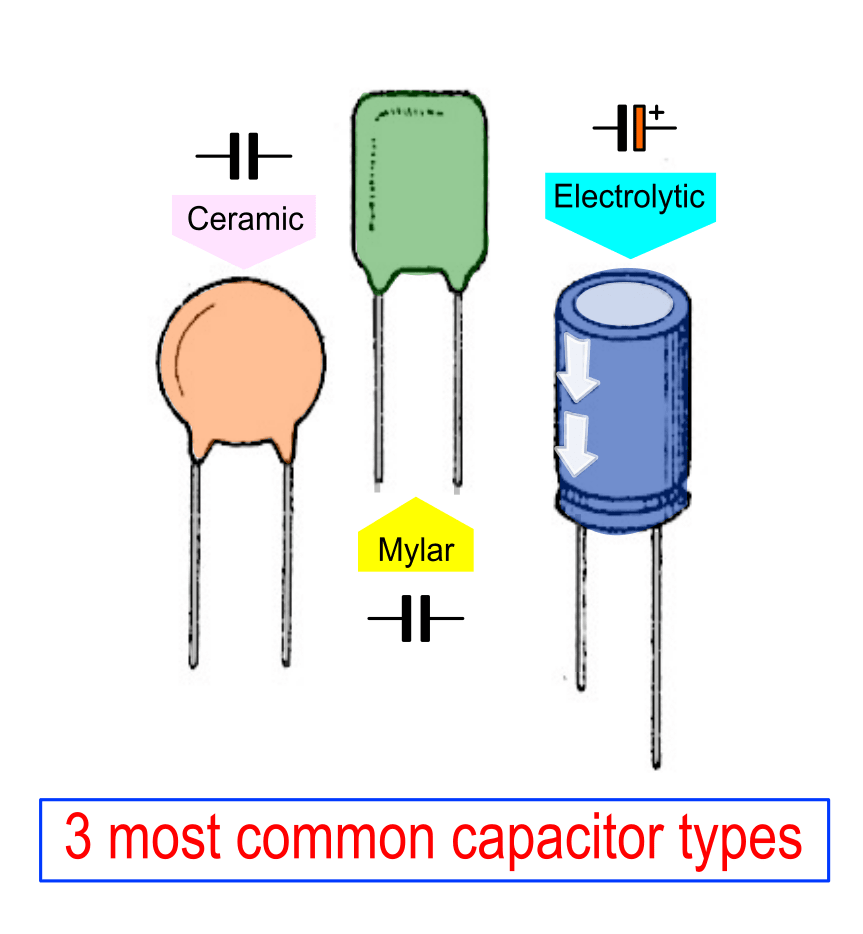
\includegraphics[width=0.9\textwidth]{figures/fig_capacitors.png}
        \end{column}
    \end{columns}
\end{frame}

\begin{frame}{Semiconductor Diodes \& Cathode Band Identification}
    \begin{columns}[c]
        \begin{column}{0.5\textwidth}
            \begin{block}{PN Junction Physics}
                \begin{itemize}
                    \item Acts as an electrical one-way check valve.
                    \item \textbf{Forward Bias ($V > V_F$):} Conduction initiates ($V_F \approx 0.7\,\text{V}$ for Silicon, $0.3\,\text{V}$ for Schottky).
                    \item \textbf{Reverse Bias:} Blocks current up to breakdown voltage $V_{BR}$.
                    \item \textbf{Physical Marking:} Silver/black band indicates the \textbf{Cathode ($K$)} terminal.
                \end{itemize}
            \end{block}
        \end{column}
        \begin{column}{0.46\textwidth}
            \centering
            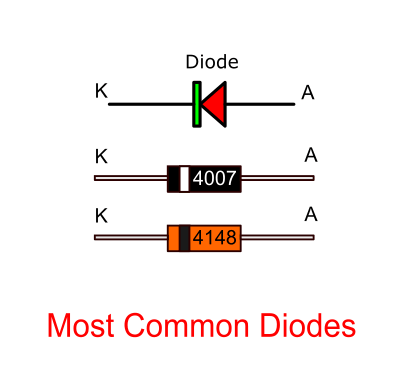
\includegraphics[width=\textwidth]{figures/fig_diodes.png}
        \end{column}
    \end{columns}
\end{frame}

\begin{frame}{Light Emitting Diodes (LEDs) \& Ballast Resistor Design}
    \begin{columns}[c]
        \begin{column}{0.52\textwidth}
            \begin{block}{Current-Limiting Formula}
                $$R = \frac{V_{CC} - V_F}{I_F}$$
                \textit{Example (5V DC Supply, Standard Red LED):}
                $$R = \frac{5.0\,\text{V} - 2.0\,\text{V}}{0.0091\,\text{A}} \approx 330\,\Omega$$
                \begin{itemize}
                    \item \textbf{Anode ($+$):} Longer lead.
                    \item \textbf{Cathode ($-$):} Shorter lead \& flat rim notch.
                \end{itemize}
            \end{block}
        \end{column}
        \begin{column}{0.44\textwidth}
            \centering
            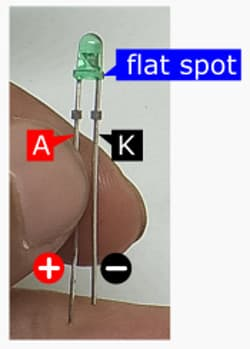
\includegraphics[height=2.4cm, keepaspectratio]{figures/fig_led_pinout.jpg}\\[0.2em]
            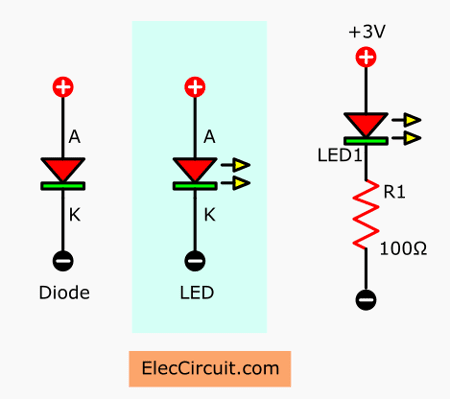
\includegraphics[height=1.8cm, keepaspectratio]{figures/fig_led_symbol.png}
        \end{column}
    \end{columns}
\end{frame}

\begin{frame}{Bipolar Junction Transistors (BJTs) \& Packaging}
    \begin{columns}[c]
        \begin{column}{0.5\textwidth}
            \begin{block}{Three-Terminal Switching}
                \begin{itemize}
                    \item Terminals: \textbf{Base (B)}, \textbf{Collector (C)}, \textbf{Emitter (E)}.
                    \item Small base current controls large collector current:
                    $$I_C = \beta I_B$$
                    \item \textbf{NPN:} Current flows Collector $\to$ Emitter when Base is positive.
                    \item Always verify pinouts (TO-92 packages vary across manufacturers: E-B-C vs. C-B-E).
                \end{itemize}
            \end{block}
        \end{column}
        \begin{column}{0.46\textwidth}
            \centering
            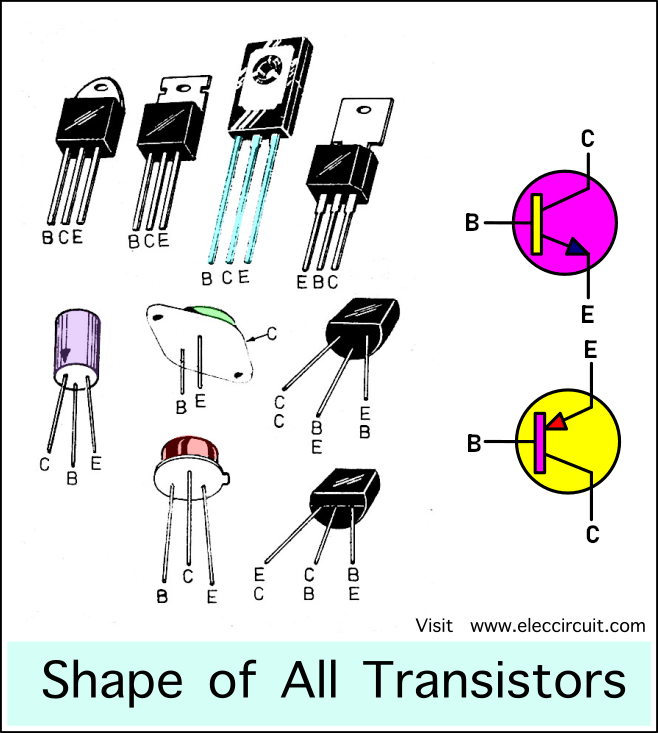
\includegraphics[width=\textwidth]{figures/fig_transistor_shapes.png}
        \end{column}
    \end{columns}
\end{frame}

\begin{frame}{Integrated Circuits (ICs) \& Dual In-Line Packaging (DIP)}
    \begin{columns}[c]
        \begin{column}{0.5\textwidth}
            \begin{block}{Pin 1 Orientation Convention}
                \begin{itemize}
                    \item \textbf{Alignment Notch:} Position the notch facing upward/leftward.
                    \item \textbf{Pin 1 Dot:} Directly adjacent to the notch.
                    \item \textbf{Counter-Clockwise Counting:} Numbering proceeds down the left column and continues up the right column.
                    \item Use IC extractors to avoid bending pins during removal.
                \end{itemize}
            \end{block}
        \end{column}
        \begin{column}{0.46\textwidth}
            \centering
            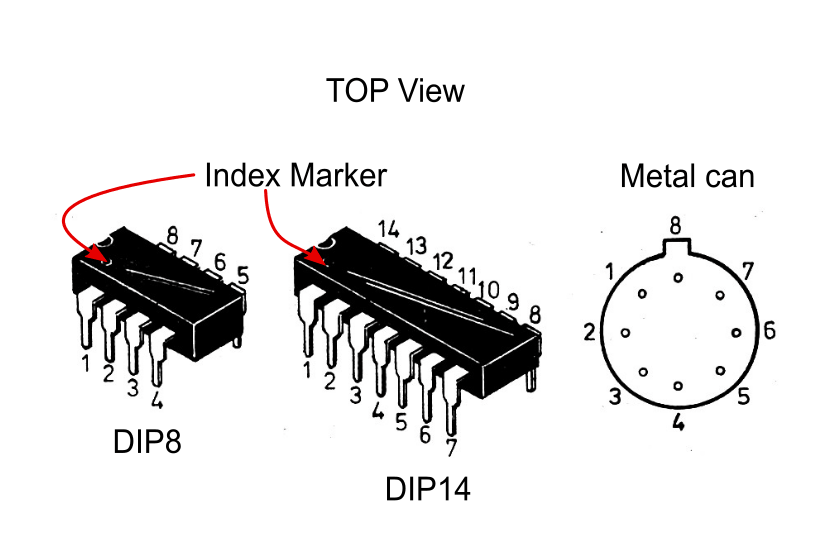
\includegraphics[width=\textwidth]{figures/fig_ic_packages.png}
        \end{column}
    \end{columns}
\end{frame}
